\documentclass[12pt,oneside,a4paper]{article}
\usepackage[utf8x]{inputenc}
\usepackage[T1]{fontenc}
\usepackage[english,polish]{babel}
\usepackage{polski}
\usepackage{listings}
\usepackage{amstext}
\usepackage{float}
\usepackage{longtable}
\restylefloat{table}
\usepackage[top=2.5cm,bottom=2.5cm,left=3.5cm,right=2.5cm]{geometry}
\usepackage{indentfirst}
\usepackage{graphicx}
\usepackage{enumitem}
\usepackage{tabularx}
\usepackage{hyperref} %spis treści niech będzie łączami
\hypersetup{
	plainpages=false,
    colorlinks,
    citecolor=black,
    filecolor=black,
    linkcolor=black,
    urlcolor=black
}
\linespread{1.3}
\setlength{\parindent}{4ex}
\begin{document}
\author{Marcin Kubik}
\author{Jacek Sosnowski}
\author{Jacek Witkowski}
\author{Piotr Zapaśnik}
\title{APSI - sklep rowerowy}
\pagenumbering{alph}
\begin{titlepage}
    \vbox to\textheight{\hyphenpenalty=10000
    \begin{center}
	\begin{tabular}{p{107mm} p{9cm}}
	    \begin{minipage}{9cm}
	      \begin{center}
	      Politechnika Warszawska \\
	      Wydział Elektroniki i~Technik Informacyjnych \\
	      Instytut Informatyki
	      \end{center}
	    \end{minipage}
	    &
	    \begin{minipage}{8cm}
	    \begin{flushleft}
	     \footnotesize
	      Rok akademicki 2013/2014
	    \vspace*{2.75\baselineskip}
	    \end{flushleft}
	    \end{minipage} \\
	\end{tabular}
	\vspace*{0.75\baselineskip}
	\par\vspace{\smallskipamount}
	{\strut Marcin Kubik\par}
	{\strut Jacek Sosnowski\par}
	{\strut Jacek Witkowski\par}
	{\strut Piotr Zapaśnik\par}
	\vspace*{1\baselineskip}{\LARGE ANALIZA I PROJEKTOWANIE SYSTEMÓW
	INFORMACYJNYCH\par}

	\vspace*{2\baselineskip}{\huge\bfseries Internetowy sklep rowerowy\par}

	\vspace*{2\baselineskip}
	\hfill\mbox{}\par\vspace*{\baselineskip}\noindent
	\begin{tabular}[b]{@{}p{3cm}@{\ }l@{}}
	    {\large\hfill } & {\large }
	\end{tabular}
	\hfill
	\begin{tabular}[b]{@{}l@{}}
	Prowadzący: \\[\smallskipamount]
	{\large mgr inż. Piotr Salata}
	\end{tabular}\par
	\vspace*{2\baselineskip}
    \begin{tabular}{p{\textwidth}}
    \end{tabular}
    \end{center}} 

\end{titlepage}
\clearpage
\tableofcontents
\pagenumbering{arabic}
\clearpage
\section{Wstęp}

Tutaj będzie wstęp\ldots
\section{Zakres realizacji}

Niniejszy rozdział prezentuje specyfikację wymagań odnośnie sposobu realizacji
projektu. Nakreślając role poszczególnych zespołów oraz główne zadania jakie
mają realizować w ramach swoich prac.

\subsection{Realizacja projektu}

Projekt jest realizowany w siedzibie firmy Bike Shop sp. z.o.o.
Umożliwi to szybkie podejmowanie decyzji w przypadku powstawania
ewentualnych niejasności a także łatwiejsze reagowanie na przeszkody,
jakie pojawiają się w czasie procesu projektowania. 
Zleceniodawca zobowiązał się do delegacji doświadczonego pracownika, który zna
specyfikę działania firmy oraz jej cele biznesowe. Ta osoba będzie uczestniczyć
w projekcie bezpośrednio na etapie analizy.

Zgodnie z dokumentem załączonym do umowy Zleceniodawca zobowiązał się do
udostępnienia firmie implementującej system pomieszczenia, w których
możliwa będzie praca zespołu projektowego. Pomieszczenia takie
powinny charakteryzować się dostępem do szybkiego łącza
internetowego. 

\subsection{Wstępny zarys technologiczny}
Tworzony przez zleceniobiorcę system zostanie stworzony w logice
trójwarstwowej umożliwiającej łatwe i wydajne zarządzanie całością
przedsięwzięcia oraz umożliwiającej dalszą modyfikację i rozbudowę.
Podział na warstwy jest następujący:

\begin{itemize}
  \item Warstwa prezentacji odpowiada za część graficzną, reprezentację danych
  przechowywanych w systemie oraz za umożliwienie użytkownikowi przeglądania
  dostępnych produktów, a także złożenie zamówienia. Osobny moduł odpowiedzialny
  jest za dostęp do administracyjnych części systemu, dostępny wyłącznie dla
  pracowników firmy Bike Shop z.o.o.
  \item Serwer aplikacji zawierający logikę tworzonego systemu, odpowiedzialny
  za zarządzanie zamówieniami, komunikację pomiędzy bazą danych oraz interfejsem
  klienckim a także wykorzystanie infrastuktury internetowej w celu zwiększenia
  wydajności
  \item Baza danych przechowująca informacje na temat wszystkich produktów
  dostępnych w sklepie, klientów posiadających swoje konta oraz składanych przez
  nich zamówieniach.
\end{itemize}

Proces projektowy systemu zostanie oparty o dwa niezależne zespoły (analityczne
i projektowe)

\subsection{Analitycy - wymagania}
Zespół ten w ramach projektu zajmuje się prowadzeniem analizy biznesowej,
badaniem potrzeb klientów, projektuje rozwiązania dla systemu. Jest
odpowiedzialny za określanie wymagań (zarówno funkcjonalnych jak i
niefunkcjonalnych). Jego zadaniem jest też dbałość o ich prawidłową realizację.

Główne zadania:

\begin{itemize}
  \item Określenie wymagań stawianych przed systemem
  \item Tworzenie specyfikacji wymagań
  \item Tworzenie planu testów
  \item Analiza środowiska systemowego
  \item Tworzenie dokumentów projektowych
  \item Odpowiedzi na wątpliwości powstałe na etapie projektowania, czy
  implementacji
\end{itemize}

\subsection{Projektanci - wymagania}
Zespół jest odpowiedzialny za stworzenie architektury nowopowstającego
systemu oraz zapisanie jej w postaci dokumentacji technicznej. Wyniki prac tego
zespołu są niezbędne dla późniejszych etapów. W czasie implementacji służą jako
wsparcie dla programistów tworzących system.

Główne zadania:

\begin{itemize}
  \item Tworzenie projektu systemu informatycznego (oddzielnie projekt
  architektury i bazy danych)
  \item Wybór technologii i metod realizacji systemu
  \item Tworzenie dokumentacji technicznej wykorzystywanej podczas implementacji
  \item Bieżące dostosowywanie wymagań do postępów prac
\end{itemize}
\newpage
\section{Wymagania}

W tej sekcji znajduje się lista wymagań jakie spełniać powinien budowany system.
Podane są one z podziałem na dwie kategorie. Pierwsza to wymagania funkcjonalne
określające funkcjonalności systemu oraz sposoby ich użycia. Druga natomist to
wymagania niefunkcjonalne, które opisują ilościowe i jakościowe warunki
działania systemu.

\subsection{Wymagania funkcjonalne}
\subsubsection{Zamówienia}

Wymagania funkcjonalne dotyczące zamówień realizowanych przez sklep:

\begin{enumerate}
  \item Prezentacja zamówień
  \item Edycja, modyfikacja
  \begin{enumerate}
    \item Dodanie lub usunięcie produktu z zamówienia
    \item Zmiana ilości produktu
  \end{enumerate}
  \item Zmiana danych zamawiającego
  \item Usunięcie zamówienia w całości
  \item Edycja formy płatności
  \begin{enumerate}
    \item Płatność gotówką
    \begin{enumerate}
      \item Koszt w złotówkach
      \item Koszt w euro
      \item Koszt w wirtualnej walucie
    \end{enumerate}
    \item Płatność przelewem
    \item Płatność ratalna oparta o system szybkich pożyczek SuperBank
    \item Możliwość wpłaty zaliczki przed wysyłką
    \item Obniżenie kosztu o naliczone rabaty i zniżki
  \end{enumerate}
  \item Wybór sposobu potwierdzenia zamówienia (faktura, paragon)
  \item Generowanie faktury pro-forma dla danego zmówienia
  \item Zarządzanie terminem dostawy
  \item Ustawianie aktualnego stanu zamówienia.
\end{enumerate}
\subsubsection{Klient}

Wymagania funkcjonalne dotyczące klientów zamawiających części w sklepie

\begin{enumerate}
  \item Dodanie nowego klienta
  \item Edycja danych klienta
  \begin{enumerate}
    \item Edycja adresu klienta
    \item Edycja adresu e-mail
  \end{enumerate}
  \item Edycja czułych danych klienta
  \begin{enumerate}
    \item Edycja hasła
    \item Edycja statusu (stały klient, nowy klient)
  \end{enumerate}
  \item Wyrejestrowanie się klienta
  \item Usunięcie klienta
\end{enumerate}

 
\subsubsection{Opis przypadków użycia - klient}

Opis przypadków użycia wyjaśniające funkcjonalności związane z zarządzaniem
klientami:

\begin{enumerate}
  \item Rejestracja klienta \\
  \begin{tabularx}{\linewidth}{ c X }
  Aktor: & Klient \\
  Opis: & Możliwość rejestracji nowego klienta.\\
  \end{tabularx}
   \begin{enumerate}
    \item Klient uruchamia stronę internetową sklepu i wybiera opcję rejestracji
    \item Klient wstawia swoje dane osobowe i wybiera domyślny model płatności
    (kartą, za pobraniem itp.)
    \item System sprawdza wstawione dane (takie same hasła, czy istnieje już
    zarejestrowany w systemie użytkownik, czy istnieje podany adres e-mail itp.)
    \item System wysyła e-mail powitalny na adres podany przez klienta
    \item W ciągu określonego, zdefiniowanego czasu klient wybiera przesłany w
    e-mailu link, stając się pełnoprawnym użytkownikiem sklepu
  \end{enumerate}
  \item Złożenie zamówienia \\
  \begin{tabularx}{\linewidth}{ c X }
  Aktor: & Klient \\
  Opis: & Przedstawienie sposobu złożenia zamówienia.\\
  \end{tabularx}
  \begin{enumerate}
    \item Klient uruchamia stronę internetową sklepu i wyszukuje interesujące go
    produkty
    \item W momencie znalezienia pasującego produktu użytkownik wybiera opcję
    dodania do koszyka
    \item Po zakończeniu wyszukiwania użytkownik wybiera opcję przejścia do kasy
    \item System sprawdza, czy użytkownik jest zalogowany. Jeśli nie, procesuje
    przypadek użycia Logowanie do Systemu
    \item System sprawdza, czy użytkownik jest stałym klientem. Jeśli tak,
    dolicza rabat do ustalonej ceny (do sumy cen poszczególnych produktów)
    \item Użytkownik wybiera sposób płatności
    \item System dodaje do wcześniej ustalonej ceny koszty wynikające ze sposobu
    płatności
    \item Użytkownik wybiera sposób dostawy (poczta, kurier, odbiór osobisty
    itp.)
    \item System dodaje do ceny koszty wynikające ze sposobu dostawy
    \item Użytkownik, po sprawdzeniu wszystkich danych, decyduje się na złożenie
    zamówienia - po tym momencie nie może już ono być cofnięte
    \item System wysyła do użytkownika e-mail potwierdzający wraz z przewidywaną
    datą realizacji zamówienia
  \end{enumerate} 
  \item Edycja danych klienta \\
  \begin{tabularx}{\linewidth}{ c X }
  Aktor: & Klient \\
  Opis: & Możliwość zmiany, uzupełnienia danych osobowych klienta.\\
  \end{tabularx}
  \begin{enumerate}
    \item Klient uruchamia witrynę internetową sklepu
    \item Klient loguje się do systemu (tylko osoba zalogowana może zmieniać
    swoje dane)
    \item Klient edytuje wybrane pozycje ze swojego opisu (adres, numer
    telefonu itp.)
    \item W przypadku zmiany hasła klient proszony jest o podanie starego jak i
    nowego (dwukrotnie) hasła
    \item Klient zatwierdza wprowadzone zmiany
    \item System wysyła na podany przez użytkownika adres e-mail (nowy, jeśli
    to adres e-mail był jedną ze zmienianych wartości) informację o zmianie.
  \end{enumerate}
  \item Wyrejestrowanie się klienta \\
  \begin{tabularx}{\linewidth}{ c X }
  Aktor: & Klient \\
  Opis: & Klient ma możliwość w każdym momencie usunąć swoje konto z systemu.\\
  \end{tabularx}
  \begin{enumerate}
    \item Klient uruchamia witrynę internetową i loguje się na swoje konto
    (przypadek użycia Logowanie Do Systemu)
    \item Klient wybiera opcję usunięcia danych
    \item System sprawdza, czy istnieją niezrealizowane (oczekujące) zamówienia.
    Jeśli tak, wyświetla się alert z informacją, czy dane zamówienie zostało już
    wcześniej opłacone
    \item Jeśli istniały już zamówienia, które zostały opłacone a nie zostały
    jeszcze zrealizowane, system zleca odesłanie określonej kwoty pieniężnej z
    powrotem na konto użytkownika (z pominięciem kosztów obsługi)
    \item Klient zostaje poproszony o podanie przyczyn swojej decyzji -
    wypełnianie jest nieobowiązkowe
    \item Dane przechowywane są przez Okres Przechowywania Danych (wymaganie
    prawne - patrz Wymagania niefunkcjonalne punkt \ref{itm:OPD}). W tym
    czasie klient może ponownie zarejestrować się w systemie bez utraty poprzednich danych
    \item W przypadku braku ponownej rejestracji dane zostają na stałe usunięte
    z firmowej bazy danych
  \end{enumerate}
  \item Usunięcie klienta \\
  \begin{tabularx}{\linewidth}{ c X }
  Aktor: & Pracownik \\
  Opis: & Klienta można usunąć administracyjnie na przykład z powodów
  naruszenia regulaminu.\\
  \end{tabularx}
  \begin{enumerate}
    \item Pracownik sklepu wyszukuje klienta o konkretnym imieniu i nazwisku
    (lub według innych kryteriów)
    \item Pracownik wybiera opcję usunięcia klienta. 
    \item Pracownik wpisuje powód, dla którego usuwa użytkownika (informacja ta
    będzie przesłana do klienta w wiadomości e-mail)
    \item Pracownik wypełnia dane dotyczące kwestii niezrealizowanych zamówień i
    nieotrzymanych płatności
    \item Obie informacji (z poprzednich 2 kroków) są przekazywane na podany
    przez użytkownika adres e-mail
    \item Dane są przechowywane przez Okres Magazynowania Danych (patrz
    Wymagania Niefunkcjonalne punkt \ref{itm:OMD}) - w tym czasie użytkownik
    może złożyć reklamację i ewentualnie odzyskać dostęp do konta
    \item Po tym czasie, jeśli prośba o przywrócenie konta nie zostanie
    pozytywnie rozpatrzona, dane są na stałe usuwane z systemu
  \end{enumerate}
\end{enumerate}
\newpage
\subsection{Wymagania niefunkcjonalne}

\begin{enumerate}
  \item Pojemność: \\ 
  System powinien mieć możliwość przechowywania danych o 100 tys.
  użytkowników 
  \item Wydajność: \\ 
  System powinien obsługiwać bez znaczącego spadku wydajności 400
  użytkowników ``jednocześnie''. Zakładając, że użytkownik będzie wymagał
  maksymalnie 20 odświeżeń widoku systemu na minutę (jedna podstrona na 3
  sekundy). System powinien działać z wydajnością 8000 odświeżeń/minutę. 
  \item System powinien być dostępny dla klientów 24 godziny na dobę 7 dni w
  tygodniu (możliwe są przerwy konserwacyjne, jednak nie dłuższe niż 4 godziny na miesiąc pracy) 
  \item Średni czas naprawy (MTTR - ang. Mean Time to Recover) na poziomie
  1~godziny
  \item System powinien umożliwiać klientom dostęp z dowolnego miejsca na
  świecie za pomocą sieci Internet oraz jego działanie powinno być niezależne od
  używanej platformy systemowo-sprzętowej użytkownika.
  \item Dane osobowe muszą być przetwarzane zgodnie z ustawą o ochronie danych
  osobowych z dnia 29 sierpnia 1997 r. 
  \item Klient powinien mieć dostęp do wszystkich swoich danych (łącznie z
  możliwością ich aktualizacji i usunięcia) zgodnie z polskim prawem
  \item Dane te powinny być chronione w zależności od ich poziomu poufności
  (dane do autoryzacji powinny być zabezpieczone przed możliwością odczytu nawet
  przez administratora) 
  \item Komunikacja pomiędzy klientem (przeglądarką internetową, aplikacją
  mobilną itp.) powinna być szyfrowana w sposób uniemożliwiający odczytanie czułych informacji
  \item System powinien mieć wbudowane procedury przeciwdziałania sytuacjom
  awaryjnym - procedury uruchamiane przez administratora
  \begin{enumerate}
    \item Procedury sprawdzenia spójności danych - po odzyskaniu sprawności, np.
    po awarii sprzętu
    \item Procedury uruchamiane w przypadku wykrycia włamania (między innymi,
    odłączenie systemu od sieci Internet, zablokowanie modyfikacji elementów
    systemu itp.)
  \end{enumerate} 
  \item System posiadać będzie hierarchię uprawnień (ról) dla użytkowników,
  przydzielanych im w celu umożliwienia korzystania z dodatkowych
  funkcjonalności
  \item System domyślnie powinien nadawać użytkownikowi uprawnienia nie większe
  niż niezbędne mu do poprawnego zamawiania produktów i zarządzania swoim
  kontem
  \item System powinien umożliwiać automatyczne wysyłanie klientowi wiadomości
  e-mail (z prośbą o potwierdzenie zmiany hasła czy akceptacji warunków rejestracji)
  \item System powinien umożliwiać użytkownikowi zmianę (w ograniczonym stopniu)
  już złożonego zamówienia (zmiana adresu przed wysyłką itp.) bez konieczności
  ingerencji pracownika sklepu
  \item System powinien być zdolny do wyświetlania informacji w wielu językach.
  Początkowo będzie to język polski i angielski. Istnieje jednak możliwość
  rozszerzenia o kolejne.
  \item \label{itm:OPD} Okres Przechowywania Danych - to czas przez który będą
  przechowywane dane użytkownika sprzed ich zmiany lub wyrejestrowania - system zapewnia
  magazynowanie tych danych co najmniej przez 7 dni.
  \item \label{itm:OMD} Okres Magazynowania Danych to czas 30 dni przez które
  system powinien przechowywać dane o klientach po usunięciu konta klienta (czas ten może się
  zmienić z powodów prawnych)
  \item \label{itm:Platnosci} System wspiera następujące formy płatności:
  \begin{enumerate}
    \item Płatność gotówką
    \item Przelew bankowy
    \item Płatność ratalna w oparciu o zewnętrzną usługę bankową
  \end{enumerate}
  Waluty: polski złoty, euro, bitcoin
  \item \label{itm:PotwierdzenieTransakcji} Forma potwierdzenia transakcji:
  faktura albo paragon
  \\
  System powinien umożliwiać generowanie tych dokumentów oraz ich wydruk.
  
\end{enumerate}

\newpage
\section{Model analityczny}

Celem stworzonego w niniejszym rozdziale modelu analitycznego jest
zdefiniowanie, jak wyglądać będzie architektura tworzonego systemu, jakie
problemy mogą być związane z poszczególnymi elementami całości i jakie kroki
można przedsięwziąć w celu zapobieżenia najczęściej występującym i najbardziej
prawdopodobnym zagrożeniom. Aby to osiągnąć, zaprezentowano różnego rodzaju
diagramy UML, które służą jako wizualna reprezentacja architektury systemu i
pozwalają na łatwiejszą analizę stanu projektu.


Przedstawiony na poniższym obrazku diagram klas reprezentuje wszystkie
wykorzystywane przez Zleceniodawcę elementy składające się na cały system.
Diagram ten ma znaczenie przede wszystkim dla deweloperów i osób zajmujących się
wytwarzaniem oprogramowania, tym niemniej powinien zostać zatwierdzony przed
przedstawicieli Zleceniodawcy - diagram klas jest bowiem punktem łączącym z
jednej strony wyobrażenie klienta o podziale funkcjonalności a z drugiej decyzje
projektowe podjęte przez zespół zajmujący się implementacją.

Diagram klas powinien obrazować zależności (agregacje, kompozycje, relację
dziedziczenia) pomiędzy poszczególnymi klasami na tyle szczegółowo, by osoby 
nieposiadające wykształcenia informatycznego i nieznające metod programowania
obiektowego mogłby zrozumieć zasadę podziału bez szczegółowych wyjaśnień. Z
tego też powodu na poniższym rysunku skoncentrowano się na powiązaniach pomiędzy
poszczególnymi klasami a nie na nazywaniu i przedstawianiu atrybutów i metod
poszczególnych klas. Nie stanowią one żadnej wartości z punktu widzenia
Zleceniodawcy a mogą stanowić ograniczenie i usztywnienie schematu dla
deweloperów, którzy lepiej znają metody dostarczania funkcjonalności i będą
mogli lepiej modyfikować schemat w zależności od potrzeb, nie naruszając
jednocześnie warunków umowy. Wszystkie atrybuty czy operacje ważne z punktu
widzenia Zleceniodawcy, które mogą mieć wpływ na ocenę projektu zostały
umieszczone na diagramie.

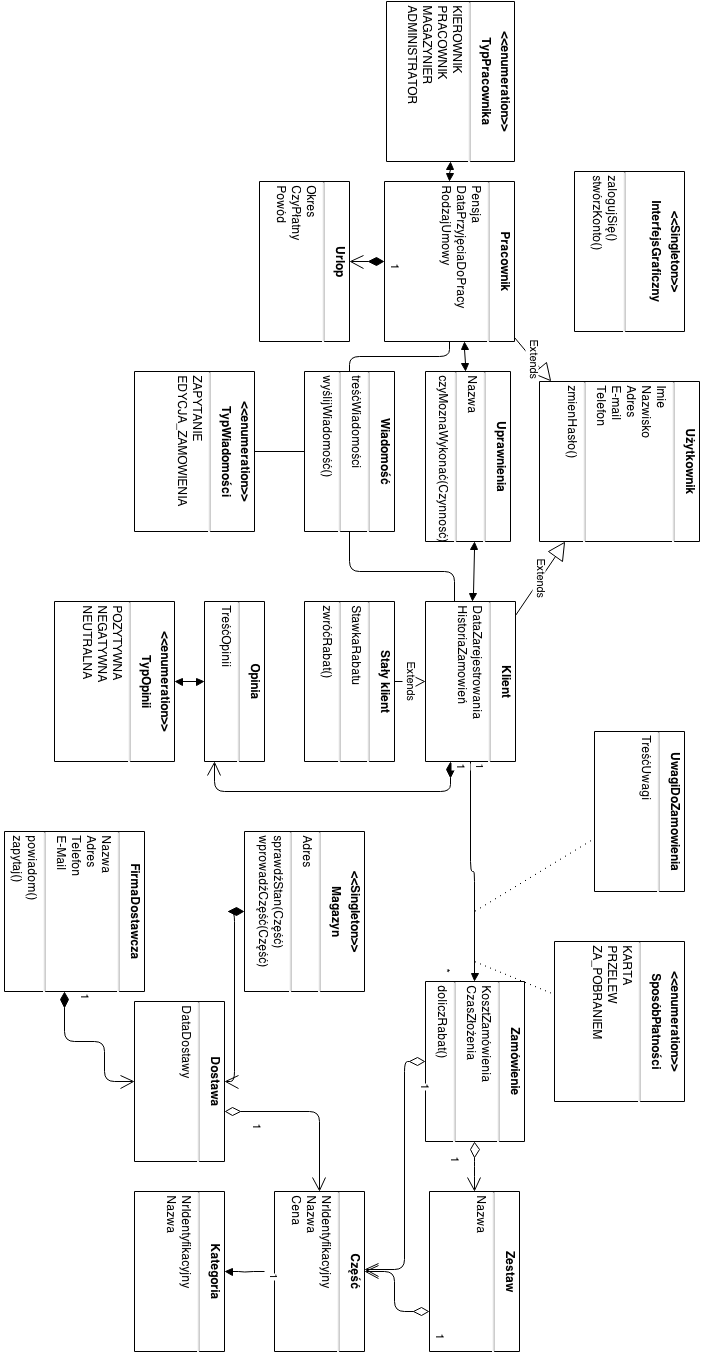
\includegraphics[width=\textwidth,
height=0.8\textheight]{graphics/ClassDiagram.png}


\newpage
Opis klas na przedstawionym diagramie:

\begin{description}
	\item[Użytkownik] \hfill \\
		Klasa abstrakcyjna, będąca bazową dla klas Klient i Pracownik, przechowuje
		informacje dotyczące danej osoby - imię, nazwisko, adres e-mail itp.
	\item[Pracownik] \hfill \\
	 	Osoba z obsługi sklepu, odpowiedzialna za realizację i zarządzanie
	 	zamówieniami
	\item[Stały klient] \hfill \\
		Osoba charakteryzująca się dużą liczbą zamówień bądź długim czasem obecności
		na stronie (czas liczony od czasu rejestracji)
	\item[Klient] \hfill \\
		Osoba składająca zamówienia w sklepie, edytująca swoje zamówienia i opłacająca
		je
	\item[Typ pracownika] \hfill \\
		Enumeracja, będąca oznaczeniem rodzaju pracownika (Szeregowy Pracownik,
		Kierownik itp.)
	\item[Urlop] \hfill \\
		Obsługa urlopów dla pracowników pod kątem czasu ich trwania, momentu ich
		rozpoczęcia (i zakończenia) itp.
	\item[Uprawnienia] \hfill \\
		Obsługa uprawnień zarówno dla pracowników jak i klientów. Pozwala na
		ustalanie, kto ma jakie uprawnienia do edycji i podglądu danych
	\item[Wiadomość] \hfill \\
		Treści przesyłane pomiędzy pracownikami i klientami, służące do przekazywania
		informacji na temat zamówień
	\item[Typ wiadomości] \hfill \\
		Enumeracja, jaki rodzaj wiadomości jest przekazywany (Zapytanie, Edycja
		Zamówienia itp.)
	\item[Opinia] \hfill \\
		Tekst na temat zamówienia, ocena poprawności i jakości realizacji zamówienia
	\item[Typ opinii] \hfill \\
		Enumeracja, jaka opinia została wydana (Pozytywna, Negatywna, Neutralna)
	\item[Zamówienie] \hfill \\
		Informacje na temat złożonego przez klienta Zamówienia
	\item[Uwagi do zamówienia] \hfill \\
		Wszelkiego rodzaju informacje, jakie klient chce zawrzeć w momencie złożenia
		zamówienia - na przykład zaznaczanie wysyłki jako prezent, ustalenie, przed
		jakim terminem zamówienie nie powinno być wysłane, czy możliwy jest odbiór
		osobisty itp.
	\item[Sposób płatności] \hfill \\
		Informacja, jak użytkownik chce zapłacić za złożone zamówienie - inaczej
		wygląda procesowanie zapłaty kartą (wysłanie następuje dopiero po wpłynięciu
		pieniędzy, opłata za pobraniem jest uiszczana dopiero po wysłaniu)
	\item[Część] \hfill \\
		Pojedyncza część rowerowa wraz z informacjami na jej temat - rozmiar, nazwa,
		cena itp.
	\item[Zestaw] \hfill \\
		Złożenie kilku części w jeden, funkcjonalnie sprawny rower. Przechowuje
		informację o tym, jakie części są wymagane, ile ma ich być (rama - 1, pedały
		-2, przerzutki - nieokreślone)
	\item[Kategoria] \hfill \\
		Informacja, do jakiej kategorii zaliczana jest dana część. Jest to pomocne do
		układania zestawów i sprawdzania ich poprawności
	\item[Dostawa] \hfill \\
		Informacje na temat jednej dostawy, jakie części i w jakiej ilości zostały
		dostarczone i kiedy
	\item[Firma dostawcza] \hfill \\
		Informacje na temat firmy, która dostarcza części - dane kontaktowe, adres
		oraz jakie części są w stanie dostarczyć
	\item[Magazyn] \hfill \\
		Klasa pozwalająca na zarządzanie częściami przechowywanymi w magazynie,
		sprawdzanie ich dostępności oraz aktualizacja stanu
	\item[Interfejs graficzny] \hfill \\
		Klasa będąca ``wejściem'' do diagramu klas, odpowiedzialna za podstawową,
		wstępną integrację z użytkownikiem
\end{description}
\end{document}